I have contributed following things in this project:
\subsection{Surcharges}
I made a Surcharge model to calculate taxes.Earlier there was no option to include taxes in Catalog. I made changes in admin.py, views.py and models.py. 
\subsection{TOTAL}
I made an option to do total of all materials and calculate taxes on it. I made a view for it in views.py in Prints App.
\subsection{Suspense App}
I and my team mate made Suspense app. We made views.py, forms.py, and templates for Suspense app.

{\bf Role in LibreHatti Software:}
This 'Total' played a great role in Software as a software without generating total for each PurchaseOrder, it would have been of no use.
Suspense App we made was of great use because It generates bill depending upon clients.

\subsection{Future scope}
There lies a great future scope in  it as bill generation can be made linked (in my project it is static). 
 There are various totalling techniques and algorithms
which could be used and were studied: 

\begin{figure}[h]
\subsection{Implementation}
\centering 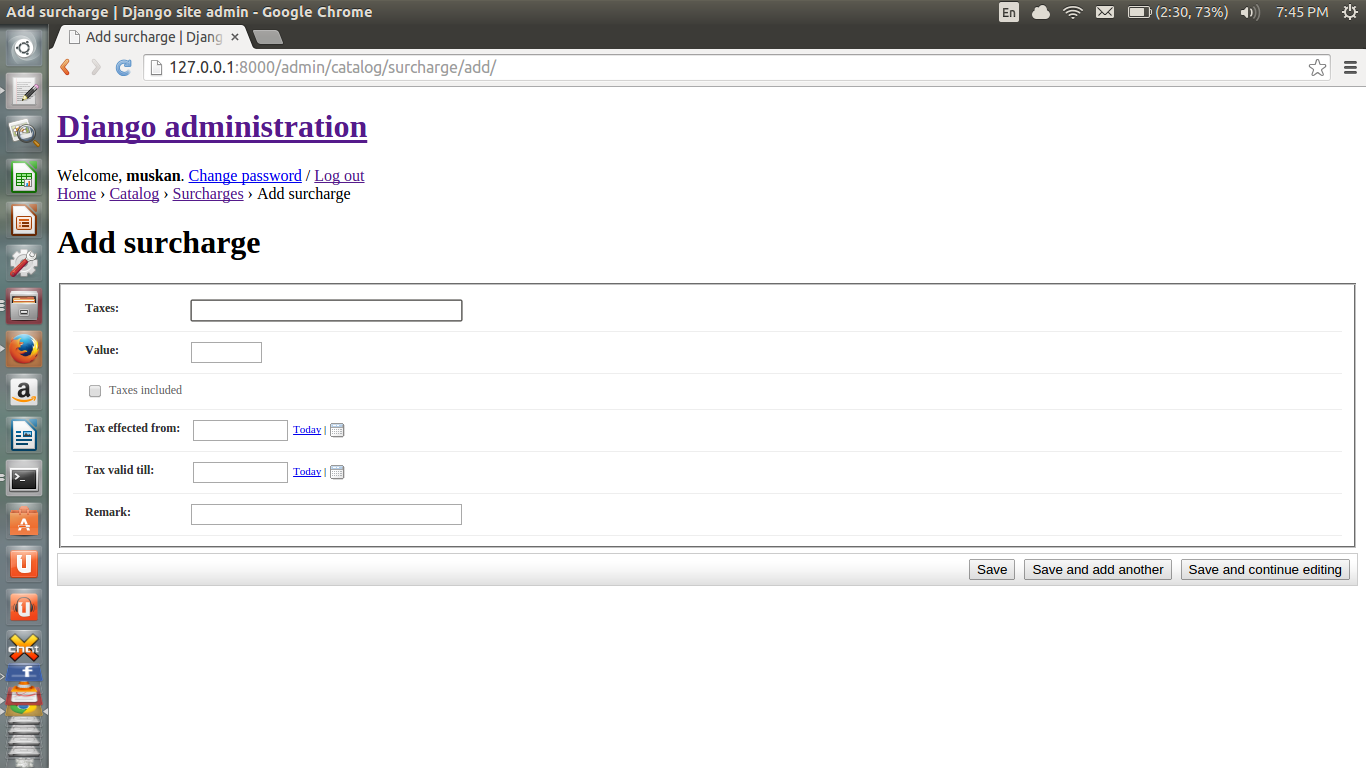
\includegraphics[scale=0.60]{images/Sur.png}
\centering 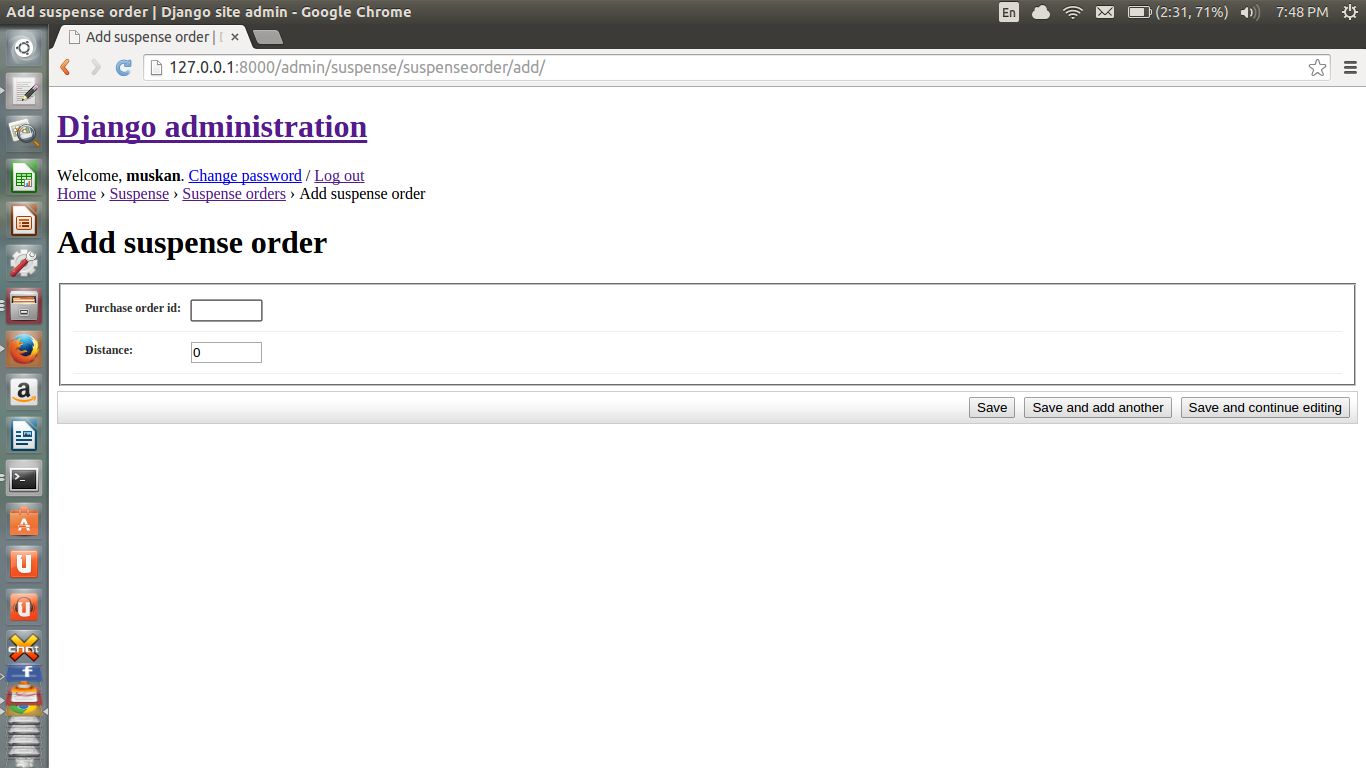
\includegraphics[scale=0.60]{images/Sus.png}
\caption{Search results}
\end{figure}
